\documentclass[12pt, openany]{report}
\usepackage[utf8]{inputenc}
\usepackage[T1]{fontenc}
\usepackage{amsmath,amsfonts,amssymb}
\usepackage{amssymb}
\usepackage{multicol}
\usepackage[a4paper,left=2.5cm,right=2.5cm,top=2.5cm,bottom=2.5cm]{geometry}
\usepackage[french]{babel}
\usepackage{libertine}
\usepackage{graphicx}
\usepackage{wrapfig}
\usepackage{float}
\usepackage{enumitem}
\usepackage[]{titletoc}
\usepackage{empheq}
\usepackage{titlesec}
\usepackage{textcomp}
\usepackage{caption}
\usepackage{tabularray}
\usepackage{subcaption}
\usepackage[bottom]{footmisc}
\usepackage{pdfpages}
\usepackage{tabularx}
\usepackage{amsthm}
\usepackage[skins]{tcolorbox}
\titleformat{\chapter}[display]
  {\normalfont\bfseries}{}{0pt}{\Huge}
\usepackage{hyperref}
\newcommand{\HRule}{\rule{\linewidth}{0.5mm}}
\usepackage{silence}
\WarningFilter{latex}{Overfull \hbox}

\begin{document}

\begin{titlepage}
    \begin{sffamily}
    \begin{center}
        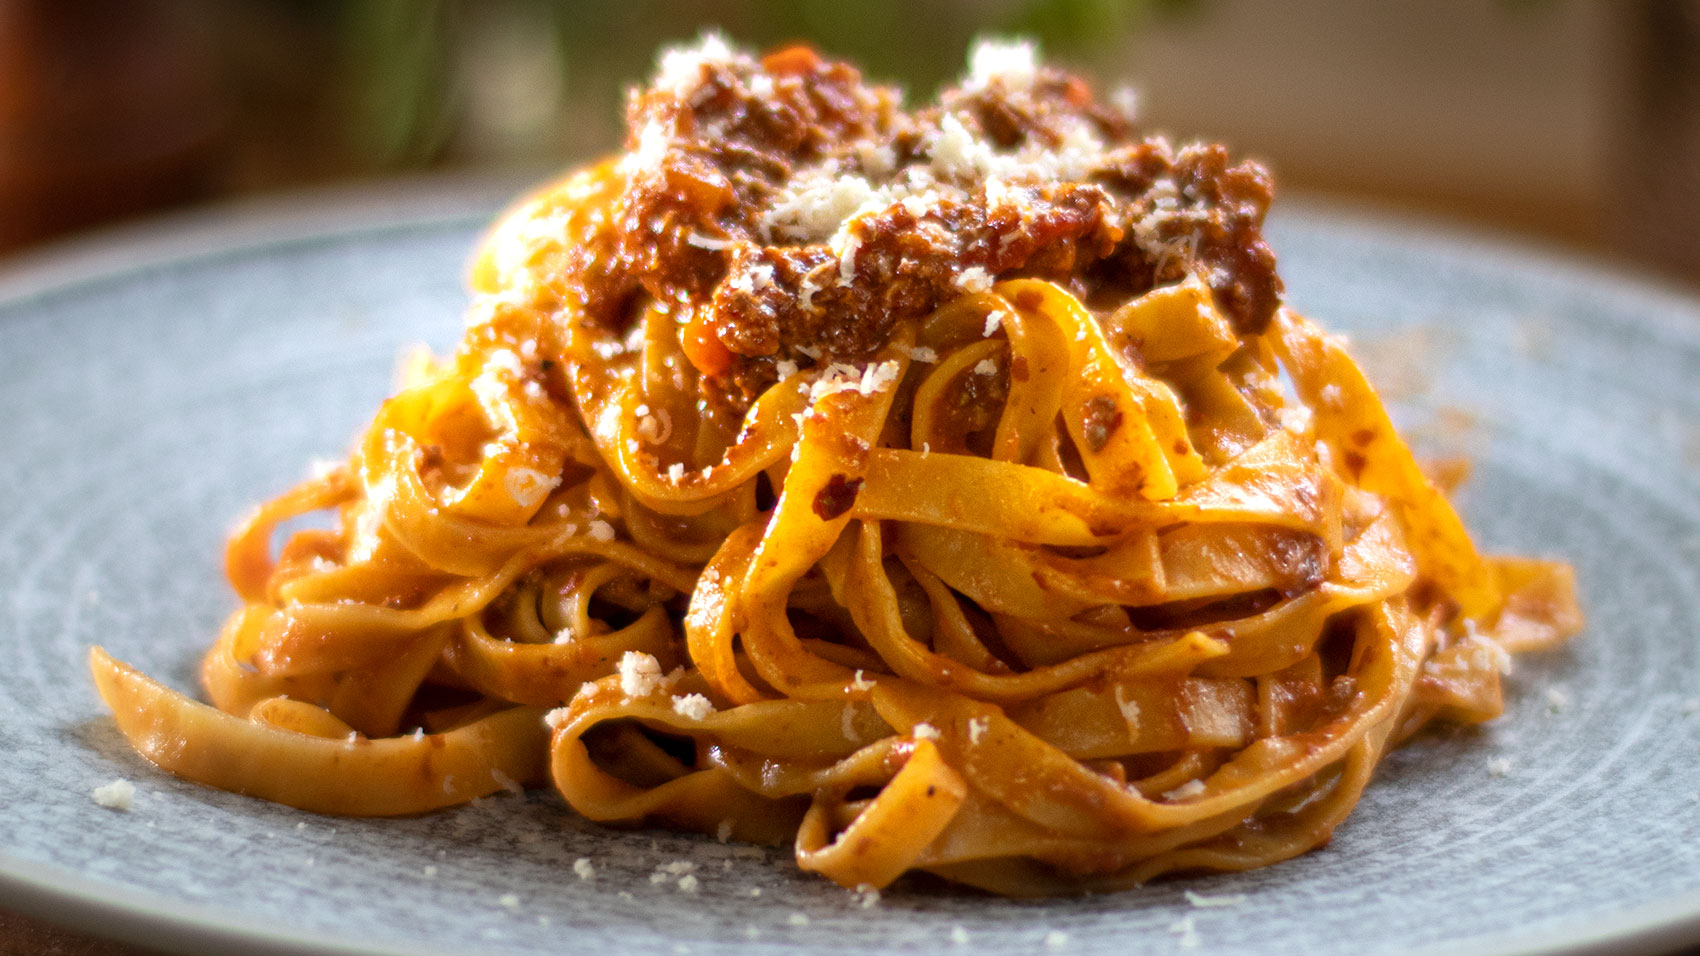
\includegraphics[scale=0.25]{img/page_de_garde.png} \\[1cm]
        \HRule \\[0.4cm]
        { \huge \bfseries LITAL1100 Italien - niveau élémentaire \\[0.4cm] }
    
        \HRule \\[1.5cm]
        \textsc{\LARGE Simon Desmidt}\\[1cm]
        \vfill
        \vspace{2cm}
        {\large Année académique 2024-2025 - Q1}
        \vspace{0.4cm}
         
        
\includegraphics[width=0.15\textwidth]{img/ilv.png}
        
        UCLouvain\\
    
    \end{center}
    \end{sffamily}
\end{titlepage}

\setcounter{tocdepth}{1}
\tableofcontents
\chapter{Conjugaison}
\section{Indicatif présent}
\subsection{Essere/Avere}
\begin{center}
    \begin{tabular}{c|c|c}
        & ESSERE & AVERE \\ \hline
        io & sono & ho\\
        tu & sei & hai\\
        lui/lei/Lei & è & ha\\ 
        noi & siamo & abbiamo \\
        voi & siete & avete \\
        loro & sono & hanno\\
    \end{tabular}
\end{center}
\subsection{Règle générale}
\begin{minipage}{.49\textwidth}
    \vspace{.75cm}
    \begin{center}
        \begin{tabular}{c||c|c|c}
            & ARE & ERE & IRE\\
            \hline
            io & -o & -o & -o\\
            tu & -i & -i & -i\\
            lui/lei/Lei & -a & -e & -e\\
            noi & -iamo & -iamo & -iamo\\
            voi & -ate & -ete & -ite\\
            loro & -ano & -ono & -ono\\
        \end{tabular}
    \end{center}
\end{minipage}
\begin{minipage}{.45\textwidth}
    Cas particuliers de spedire (envoyer), preferire (péférer), finire (finir) et capire (comprendre):
    \begin{center}
        \begin{tabular}{c||c}
            io & -isco \\
            tu & -isci \\
            lui & -isce \\
            noi & -iamo \\
            voi & -ite \\
            loro & -iscono \\
        \end{tabular}
    \end{center}
\end{minipage}
\subsection{Cas particuliers}
\begin{minipage}{.315\textwidth}
    \begin{center}
        \begin{tabular}{c||c}
            & FARE\\ \hline
            io & faccio\\
            tu & fai\\
            lui & fa\\
            noi & facciamo\\
            voi & fate\\
            loro & fanno\\
        \end{tabular}
    \end{center}
\end{minipage}
\begin{minipage}{.315\textwidth}
    \begin{center}
        \begin{tabular}{c||c}
            & ANDARE\\ \hline
            io & vado\\
            tu & vai\\
            lui & va\\
            noi & andiamo\\
            voi & andate\\
            loro & vanno\\
        \end{tabular}
    \end{center}
\end{minipage}
\begin{minipage}{.315\textwidth}
    \begin{center}
        \begin{tabular}{c||c}
            & VENIRE\\ \hline
            io & vengo\\
            tu & vieni\\
            lui & viene\\
            noi & veniamo\\
            voi & venite\\
            loro & vengono\\
        \end{tabular}
    \end{center}
\end{minipage}
\begin{minipage}{.33\textwidth}
    \begin{center}
        \begin{tabular}{c||c}
            & STARE\\ \hline
            io & sto\\
            tu & stai\\
            lui & sta\\
            noi & stiamo\\
            voi & state\\
            loro & stanno\\
        \end{tabular}
    \end{center}
\end{minipage}
\begin{minipage}{.33\textwidth}
    \begin{center}
        \begin{tabular}{c||c}
            & USCIRE (sortir)\\ \hline
            io & esco\\
            tu & esci\\
            lui & esce\\
            noi & usciamo\\
            voi & uscite\\
            loro & escono\\
        \end{tabular}
    \end{center}
\end{minipage}
\begin{minipage}{.33\textwidth}
    \begin{center}
        \begin{tabular}{c||c}
            & DIRE\\ \hline
            io & dico\\
            tu & dici\\
            lui & dice\\
            noi & diciamo\\
            voi & dicite\\
            loro & dicono\\
        \end{tabular}
    \end{center}
\end{minipage}
\subsection{Verbes réfléchis}
Les verbes réfléchis fonctionnent comme les réguliers, avec les pronoms réfléchis en plus:
\begin{center}
    \begin{tabular}{c||c|c|c|c}
        & & ARE & ERE & IRE\\
        \hline
        io & mi & -o & -o & -o\\
        tu & ti & -i & -i & -i\\
        lui/lei/Lei & si & -a & -e & -e\\
        noi & ci & -iamo & -iamo & -iamo\\
        voi & vi & -ate & -ete & -ite\\
        loro & si &-ano & -ono & -ono\\
    \end{tabular}
\end{center}
\subsection{Volere/Potere/Dovere}
\begin{minipage}{.315\textwidth}
    \begin{center}
        \begin{tabular}{c||c}
            & VOLERE \\ \hline
            io & voglio\\
            tu & vuoi\\
            lui & vuole\\
            noi & vogliamo\\
            voi & volete \\
            loro & vogliono \\
        \end{tabular}
    \end{center}
\end{minipage}
\begin{minipage}{.315\textwidth}
    \begin{center}
        \begin{tabular}{c||c}
            & POTERE \\ \hline
            io & posso \\
            tu & puoi \\
            lui & può\\
            noi & possiamo\\
            voi & potete\\
            loro & possono\\
        \end{tabular}
    \end{center}
\end{minipage}
\begin{minipage}{.315\textwidth}
    \begin{center}
        \begin{tabular}{c||c}
            & DOVERE \\ \hline
            io & devo/debbo\\
            tu & devi \\
            lui & deve \\
            noi & dobbiamo \\
            voi & dovete \\
            loro & devono/debbono\\
        \end{tabular}
    \end{center}
\end{minipage}
\section{Gérondif}
\begin{center}
    \begin{tabular}{c|c|c}
        ARE & ERE & IRE\\ \hline 
        -ando & -endo & -endo\\
    \end{tabular}
\end{center}
Le gérondif sert à former "Stare + gérondif", i.e. "être en train de".
\section{Impératif}
\begin{center}
    \begin{tabular}{c|c|c|c}
        & ARE & ERE & IRE\\ \hline
        tu & -a & -i & -i \\
        noi & -iamo & -iamo & -iamo \\
        voi & -ate & -ete & -ite \\
    \end{tabular}
\end{center}
\begin{itemize}
    \item [$\rightarrow$] Remarque : la seule différence se situe au tu pour les verbes en ARE. 
\end{itemize}
La forme négative est la même pour noi et voi. Elle est "non + infinitif" au tu. 
\subsection{Cas particuliers}
\begin{center}
    \begin{tabular}{c|c}
        vai & va'\\
        fai & fa'\\
        stai & sta'\\
        dai (dare = donner) & da'\\
        dici (dire = dire) & di'\\
        essere & sii/cerca di essere (à l'oral)\\
        avera & abbi\\ 
    \end{tabular}
\end{center}
Quand l'impératif est utilisé avec un pronom (e.g. change-la!), on fusionne le verbe et le pronom, e.g. compraLA, leggiamoLO, apriteLE. 
\section{Imparfait}
\begin{center}
    \begin{tabular}{c|c|c|c}
        & ARE & ERE & IRE\\ \hline
        io & -avo & -evo & -ivo\\
        tu & -avi & -evi & -ivi\\
        lui & -ava & -eva & -iva\\
        noi & -avamo & -evamo & -ivamo\\
        voi & -avate & -evate & -ivate\\
        loro & -avano & -evano & -ivano\\
    \end{tabular}
\end{center}
\begin{itemize}
    \item [$\rightarrow$] Remarque : tous les irréguliers deviennent réguliers, sauf cas rares.
\end{itemize}
\subsection{Cas rares}
\begin{minipage}{.315\textwidth}
    \begin{center}
        \begin{tabular}{c||c}
            & ESSERE \\ \hline
            io & ero \\
            tu & eri \\
            lui & era \\
            noi & eravamo \\
            voi & eravate \\
            loro & erano \\
        \end{tabular}
    \end{center}
\end{minipage}
\begin{minipage}{.315\textwidth}
    \begin{center}
        \begin{tabular}{c||c}
            & FARE \\ \hline
            io & facevo \\
            tu & facevi \\
            lui & faceva \\
            noi & facevamo\\
            voi & facevate\\
            loro & facevano \\
        \end{tabular}
    \end{center}
\end{minipage}
\begin{minipage}{.315\textwidth}
    \begin{center}
        \begin{tabular}{c||c}
            & DIRE \\ \hline
            io & dicevo \\
            tu & dicevi \\
            lui & diceva \\
            noi & dicevamo\\
            voi & dicevate \\
            loro & dicevano\\
        \end{tabular}
    \end{center}
\end{minipage}
\section{Passé composé}
TODO
\section{Futur simple}
\subsection{Règle générale}
\begin{center}
    \begin{tabular}{c|c|c|c}
        & ARE & ERE & IRE\\ \hline
        io & -erò & -erò & -irò\\
        tu & -erai & -erai & -irai\\
        lui & -erà & -erà & -irà\\
        noi & -eremo & -eremo & -iremo\\
        voi & -erete & -erete & -irete\\
        loro & -eranno & -eranno & -iranno\\
    \end{tabular}
\end{center} 
\subsection{Cas particuliers}
\begin{minipage}{.478\textwidth}
    \begin{center}
        \begin{tabular}{c|c|c}
            Français & Infinitif & Première personne \\ \hline 
            Être & Essere & sarò\\ 
            Avoir & Avere & avrò\\
            Aller & Andare & andrò\\
            Devoir & Dovere & dovrò\\
            Pouvoir & Potere & potrò\\
            Savoir & Sapere & saprò\\
            Voir & Vedere & vedrò\\
            
        \end{tabular}
    \end{center}
\end{minipage}
\begin{minipage}{.478\textwidth}
    \begin{center}
        \begin{tabular}{c|c|c}
            Français & Infinitif & Première personne \\ \hline
            Vivre & Vivere & vivrò\\
            Boire & Bere & berrò\\
            Venir & Venire & verrò\\ 
            Vouloir & Volere & vorrò\\
            Dire & Dire & dirò\\
            Faire & Fare & farò\\
            Être & Stare & starò\\
        \end{tabular}
    \end{center}
\end{minipage}
\begin{itemize}
    \item [$\to$] Remarque : les verbes en -care et -gare ont un h (gherò, cherò).
\end{itemize}
\subsection{Expressions de temporalité}
\begin{center}
    \begin{tabular}{c|c|c|c}
        \multicolumn{2}{c|}{\textbf{Futur}} & \multicolumn{2}{c}{\textbf{Passé}} \\ \hline
        Domani & Demain & Ieri & Hier \\
        Dopodomani & Après-demain & L'altroieri & Avant-hier \\
        Fra/tra due giorni & Dans deux jours & Due giorni fa & Il y a deux jours \\
        La settimana prossima & La semaine prochaine & La settimana scorsa & La semaine passée \\
        Domani mattina & Demain matin & Ieri mattina & Hier matin \\
        Domani sera/notte & Demain soir & Ieri sera & Hier soir \\
    \end{tabular}
\end{center}
\section{Futur antérieur}
\begin{center}
    Essere/Avere (futur simple) + Participe passé 
\end{center}
\begin{itemize}
    \item [$\to$] Remarque : l'utilisation est la même qu'en français.
\end{itemize}
\chapter{Grammaire}
\section{Terminaisons des noms et adjectifs}
\begin{center}
    \begin{tabular}{c|c|c}
        Singulier & Pluriel & Cas\\
        \hline
        -o & -i & Masculin \\
        -a & -e & Féminin \\
        -e & -i & Masculin ou féminin\\
    \end{tabular}
\end{center}
L'adjectif vient en général après le nom 
\section{Déterminants}
\begin{center}
    \begin{tabular}{c|c|c|c|c}
        \multicolumn{2}{c|}{Déterminés} & \multicolumn{2}{c|}{Indéterminés} & \\ \hline
        Singulier & Pluriel & Singulier & Pluriel & \\
        La & Le & Una & Delle & Féminin commençant par une consonne \\ 
        L' & Le & Un' & Delle & Féminin commençant par une voyelle \\ 
        Lo & Gli & Uno & Degli & Masculin commençant par s+consonne, xyz, psi, etc\\ 
        L' & Gli & Un & Degli & Masculin commençant par une voyelle \\ 
        Il & I & Un & Dei & Masculin \\ 
    \end{tabular}    
\end{center}
\section{Prépositions}
\subsection{Prépositions utilisées avec l'article}
\begin{figure}[H]
    \centering
    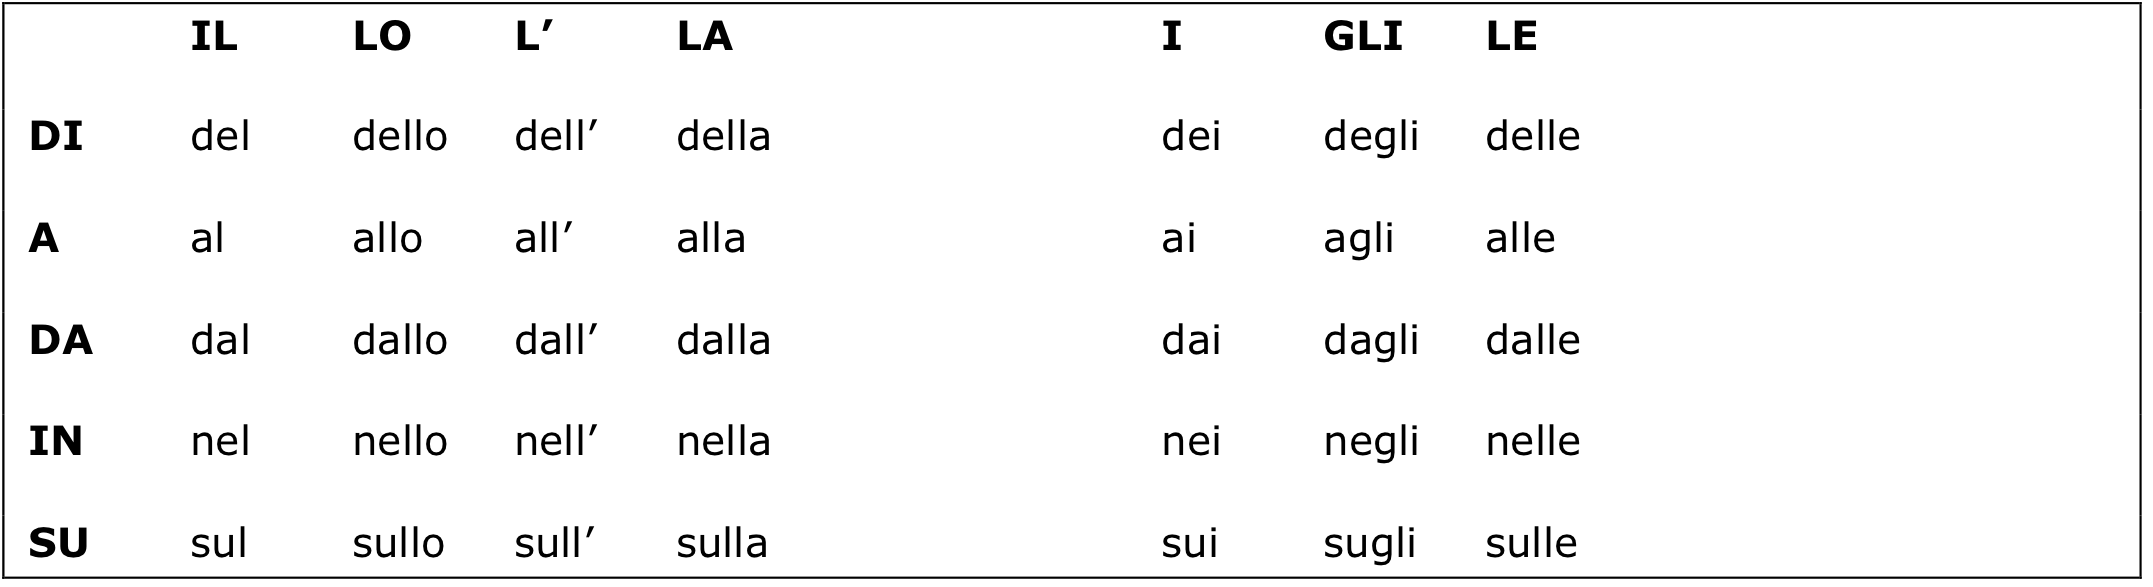
\includegraphics[width = \textwidth]{img/prep.png}
\end{figure}
Les prépositions con, per, tra, fra sont utilisées avec article séparé. 
\section{Adjectifs et pronoms possessifs}
\begin{center}
    \begin{tabular}{c|c}
        Pronom & Correspondance\\ \hline
        il mio/ il tuo/ il suo/ il nostro/ il vostro/ il loro & uno \\
        la mia/ la tua/ la sua/ la nostra/ la vostra/ la loro & una\\
        i miei/ i tuoi/ i suoi/ i nostri/ i vostri/ i loro & i\\
        le mie/ le tue/ le sue/ le nostre/ le vostre/ le loro & le\\
    \end{tabular}
\end{center}
\begin{itemize}
    \item [$\rightarrow$] Remarque : on ne met pas l'article s'il s'agit d'un membre de la famille au singulier, SAUF pour loro. 
\end{itemize}
\chapter{Divers}
\underline{Fichiers :}
\begin{itemize}
    \item \texttt{preposizioni riassunto}
    \item \texttt{Espressioni con Essere Fare Avere}
    \item Molto, troppo, poco s'accordent avec le nom quand ils sont adjectifs. 
\end{itemize}
\section{Heure}
\begin{center}
    \begin{tabular}{c|c}
        è mezzogiorno  & il est midi\\
        è mezzanotte & il est minuit\\
        è l'una & il est 1h\\
        sono le X & il est Xh (X>1)\\
        sono le X meno Y & il est Xh moins Y.\\
        sono le X e Y & il est XhY.\\
        sono le X e mezza/o & il est Xh30.\\
        sono le X e un quarto & il est Xh15.\\
        sono le X di mattina & il est Xh du matin.\\
        sono le X di sera & il est Xh du soir.\\
        sono le X in punto & il est Xh pile.\\
    \end{tabular}
\end{center}
\end{document}